\chapter{Criptografia}
\label{cryptograhy}

%
A criptografia é a ciência dos códigos secretos, permitindo a confidencialidade de uma comunicação que utiliza um meio inseguro \cite{vauldenay}. A necessidade de manter informações em sigilo impulsionou a evolução dos estudos da criptografia. O exato início da criptografia é incerto, mas na Renascença, assim como outros em muitos outros campos, o estudo da criptografia começou a ser aprofundado e suas técnicas armazenadas e ensinadas \cite{donald-davies}.

%
Uma das primeiras formas de criptografia utilizada foi a substituição de caracteres. A substituição primeiramente era feita de forma fixa, ou seja, era usada uma única tabela em que as letras do alfabeto eram trocadas por outras letras. Leon Battista Alberti introduziu uma maneira diferente de fazer a substituição, criando o algoritmo \textit{polyalphabetic substitution}. O princípio desse algoritmo era a criação de várias tabelas de substituição e a utilização de uma chave para definir a ordem que cada tabela seria usada para cifrar cada letra do texto em claro. O conjunto de tabelas de substituição é chamado de \textit{Vigenere tableau}.


%
Durante a II Guerra Mundial, informações relacionadas às estratégias de guerra deveriam ser mantidas em sigilo. Para isso, duas máquinas foram criadas e merecem destaque: a \textit{Enigma} e a \textit{Lorenz SZ40}. A máquina \textit{Enigma} foi baseada nas capacidades criptográficas de uma série de motores conectados por fio e \textit{plugboard} \cite{jennifer-wilcox}. O \textit{plugboard} fazia a substituição de uma letra por outra letra. 
\begin{figure}[h]
\centering
  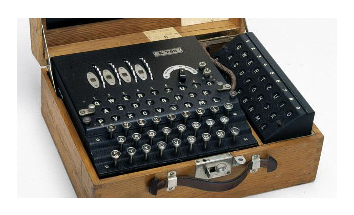
\includegraphics[keepaspectratio=true,scale=2]
  {figuras/enigma.eps}
  \caption[{Máquina Enigma}]{Máquina Enigma\protect\footnotemark}
  \label{enigma-machine}
\end{figure}
\footnotetext{Disponível e adaptado de: \url{http://www.bbc.co.uk/history/topics/enigma}}

A máquina \textit{Lorenz} foi um impressor anexado que automaticamente cifrava o texto em claro digitado pelo operador e enviava o texto cifrado por um fio de comunicação. No outro lado da comunicação, tinha uma máquina \textit{Lorenz} idêntica que fazia a decifração automaticamente e imprimia o texto em claro no papel \cite{chris-collins}.

\begin{figure}[h]
  \centering
  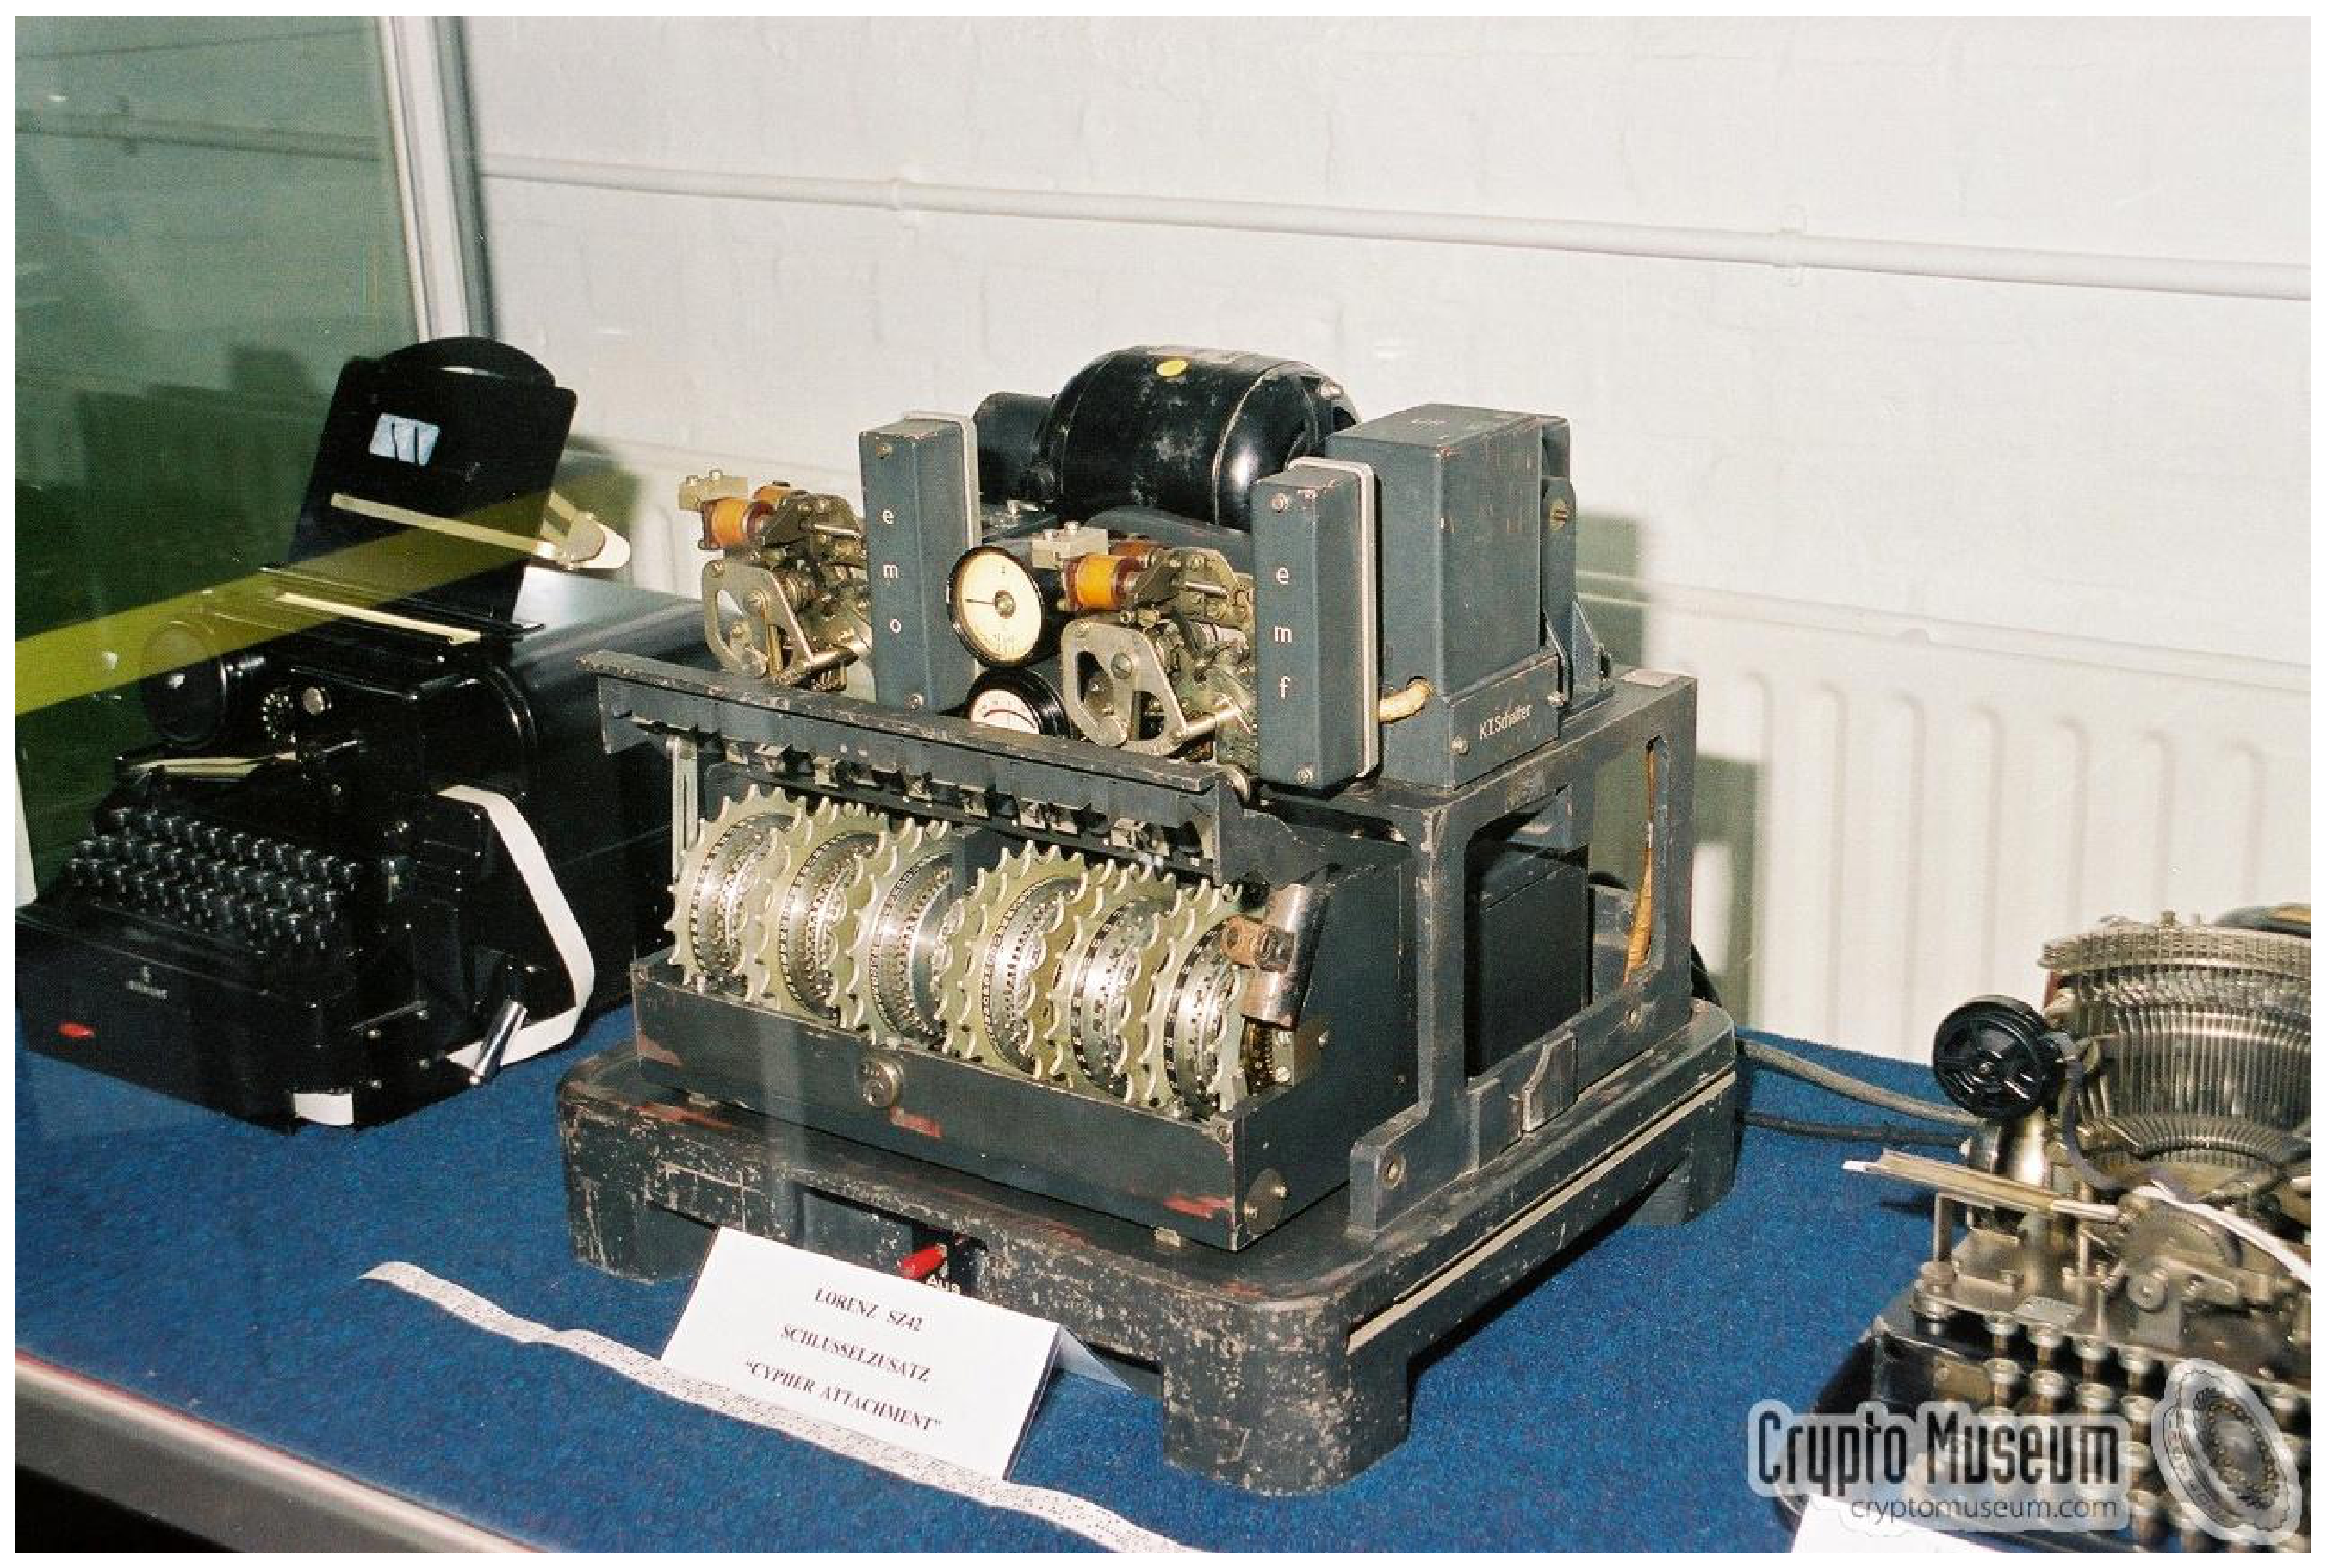
\includegraphics[keepaspectratio=true,scale=0.2]
  {figuras/sz40.eps}
  \caption[{Máquina SZ40}]{Máquina SZ40\protect\footnotemark}
    \label{sz40-machine}
\end{figure}
\footnotetext{Disponível e adaptado de: \url{http://www.cryptomuseum.com/crypto/lorenz/sz40/}}

Após a guerra, a publicação do algoritmo \textit{DES} serviu de incentivo para cientistas do mundo todo aprofundarem suas pesquisas em novos algoritmos. Nos dias de hoje existem duas linhas de estudo sobre a criptografia, a criptografia com chave simétrica e a com chave assimétrica. 


\section{Criptografia de Chave Simétrica}
\label{symmetric-cryptography}

A criptografia simétrica utiliza a mesma chave\footnote{Entrada para as funções cifrar e decifrar, é usada para que duas pessoas consigam se comunicar em segredo.} para cifrar\footnote{Função que tem como objetivo transformar uma mensagem que deve estar em sigilo e transformá-la em algo ininteligível.} e decifrar\footnote{Função que transforma uma mensagem ininteligível para a mensagem original.} uma mensagem. É objeto de estudo para muitos cientistas e existem muitos algoritmos que ainda são utilizados pelo mundo. Sua vantagem é que o custo para ser utilizada não é tão elevado e sua possibilidade de uso é maior.

\begin{figure}[h]
\centering
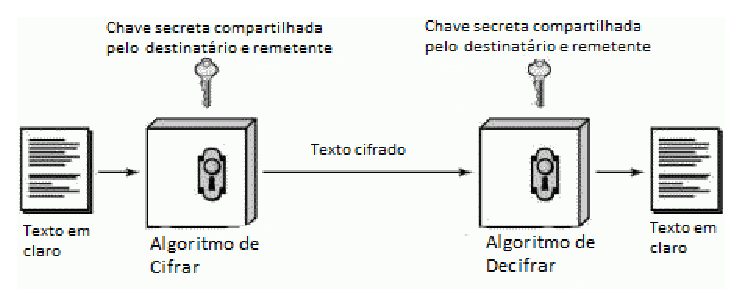
\includegraphics[scale=0.9]
{figuras/SymmetricCipher.eps}
\caption[Funcionamento básico da criptografia simétrica] {Funcionamento básico da criptografia simétrica\protect\footnotemark}
\end{figure}

\footnotetext{Disponível e adaptado de: \url{http://www.codeproject.com/Articles/21076/Securing-Data-in-NET}}
Os algoritmos são divididos em: cifra de bloco e cifra de fluxo.

\subsection{Cifra de Bloco}
\label{block-cipher}

A cifra de bloco tem como princípio a cifra de blocos de caracteres com tamanho definido e a mensagem criptografada deve ter o mesmo tamanho da mensagem em claro. Um algoritmo muito conhecido é o \textit{DES} que foi desenvolvido pela \textit{IBM}. Foi a primeira cifra comercialmente desenvolvida e sua estrutura foi divulgada por completo \cite{alex-biryukov}. 

O tamanho da chave utilizada no \textit{DES} é considerado um problema nos dias atuais. Muitos pesquisadores sabendo desse problema tentaram remediá-lo com novas variantes criptográficas. Um exemplo é o \textit{3-DES} que utiliza duas chaves no processo, mas que, como consequência, tem seu desempenho prejudicado. 

Outra medida tomada para contornar o problema de ataques ao \textit{DES} foi a publicação de um concurso do \textit{NIST} para a escolha de um novo padrão criptográfico. Assim surgiu o \textit{AES}, que é um algoritmo que utiliza o sistema de permutação e substituição, tem o tamanho do bloco fixo de 128 bits e tamanho de chave variável entre 128, 192 ou 256 \textit{bits}. 

Existem operações que podem ser aplicadas nas cifras de blocos e que podem ser utilizadas nos algoritmos \textit{DES} e \textit{AES} para a produção de mensagens criptografadas mais seguras, são elas:

\begin{description}
\item [ECB] a mensagem é dividida em blocos e consiste em cifrar os blocos de forma independente um do outro e com uma chave fixa. A desvantagem desse modo de cifra é que blocos de texto em claro iguais produzem blocos de texto cifrado iguais.
\begin{figure}[h]
\centering
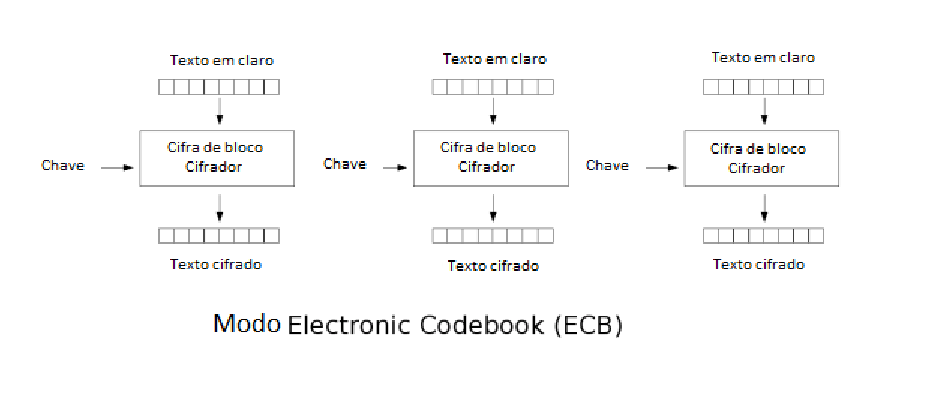
\includegraphics[keepaspectratio=true,scale=0.8]
	{figuras/ecb.eps}
	\caption[Modo Electronic Codebook]{Modo \textit{Electronic Codebook}\protect\footnotemark}
	
\end{figure} 
\footnotetext{Disponível e adaptado de: \url{http://cryptodox.com/Block\_cipher\_modes\_of\_operation}}
\item[CBC] a mensagem é dividida em blocos e o modo de cifra utiliza da operação de ou-exclusivo entre um vetor de inicialização (para o primeiro bloco) e o texto em claro\footnote{Mensagem que deve ser mantida em sigilo e que se deseja cifrar.} e por fim um ou-exclusivo do resultado com a chave. A partir do segundo bloco, ao invés de um vetor de inicialização, é utilizado o bloco criptografado anterior.
\begin{figure}[h]
\centering
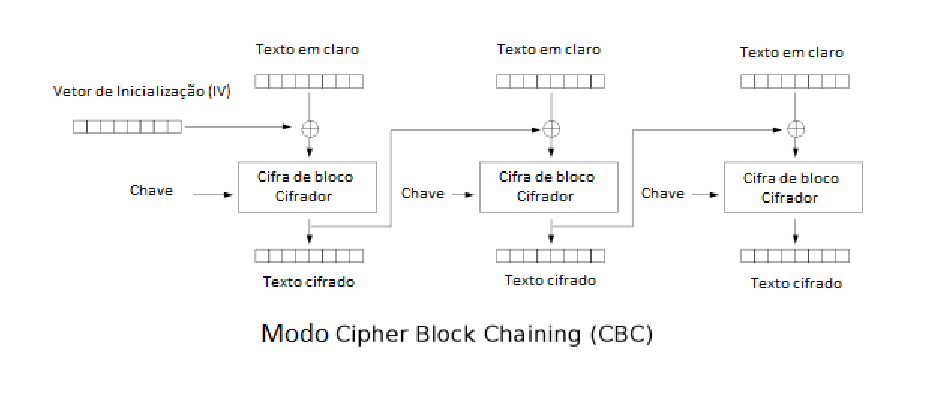
\includegraphics[keepaspectratio=true,scale=0.8]
    {figuras/cbc.eps}
    \caption[Modo Cipher Block Chaining]{Modo \textit{Cipher Block Chaining}\protect\footnotemark}
\end{figure} 
\footnotetext{Disponível e adaptado de:\url{https://www.adayinthelifeof.nl/2010/12/08/encryption-operating-modes-ecb-vs-cbc/}}
%rever
\item[CFB] a mensagem também é dividida em blocos e esse modo de cifra é muito similar ao \textit{CBC}, porém é feito um ou-exclusivo da chave com o vetor de inicialização, o bloco criptografado anterior e com o resultado é feito um ou-exclusivo com a mensagem em claro.
\begin{figure}[h]
\centering
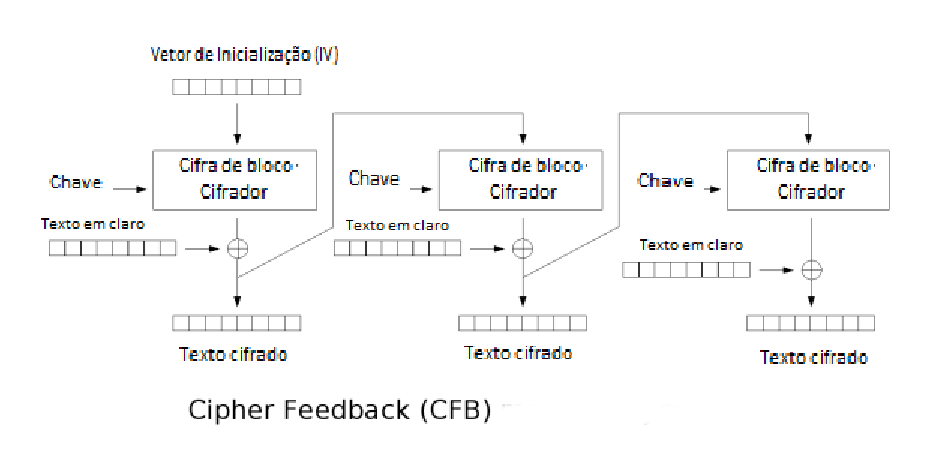
\includegraphics[keepaspectratio=true,scale=0.8]
    {figuras/cfb.eps}
    \caption[Modo Cipher Feedback]{Modo \textit{Cipher Feedback} \protect\footnotemark} 
\end{figure}
\footnotetext{Disponível e adaptado de: \url{http://crypto.stackexchange.com/questions/2476/cipher-feedback-mode}}
\item[OFB] a diferença em relação ao CFB é que o resultado entre o vetor de inicialização e a chave ou resultado da operação anterior e a chave, serve de entrada para o próximo bloco, ao invés do bloco criptografado.
\begin{figure}[h]
\centering
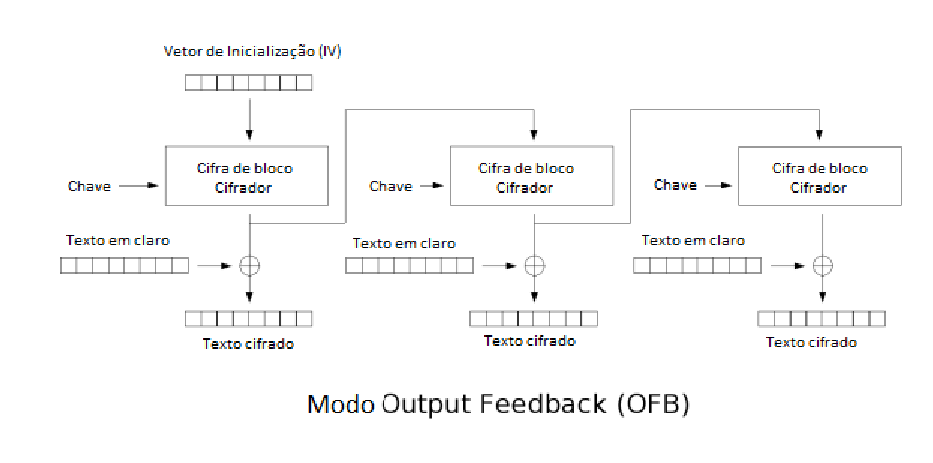
\includegraphics[keepaspectratio=true,scale=0.8]
    {figuras/ofb.eps}
    \caption[Modo Output Feedback]{Modo \textit{Output Feedback}\protect\footnotemark} 
\end{figure}
\footnotetext{Disponível e adaptado de: \url{http://commons.wikimedia.org/wiki/File:Ofb\_decryption.png}}
\item[CTR] utiliza como entrada para a função criptográfica um contador que é acrescentado de um em um. 
\begin{figure}[h]
\centering
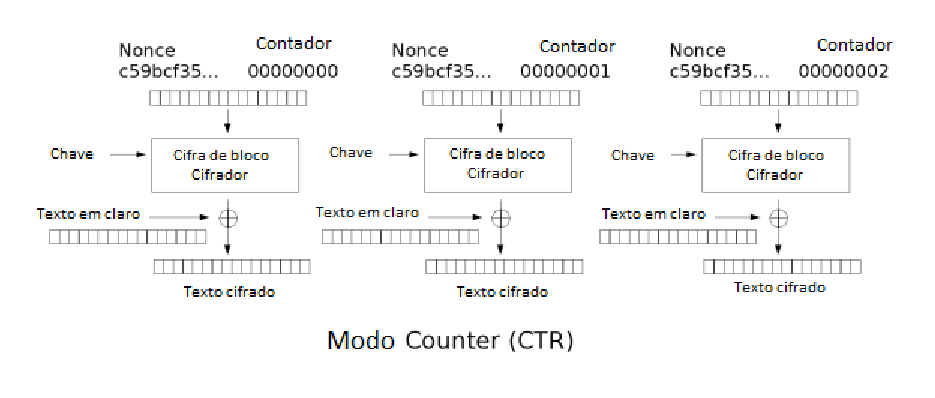
\includegraphics[keepaspectratio=true,scale=0.8]
    {figuras/ctr.eps}
    \caption[Modo Counter]{Modo \textit{Counter}\protect\footnotemark} 
\end{figure}
\footnotetext{Disponível e adaptado de: \url{http://crypto.stackexchange.com/questions/8151/counter-mode-static-iv-but-different-keys}}
\end{description}

\subsubsection{Algoritmo DES}

Como dito anteriormente, o DES foi o primeiro algoritmo que foi publicado e utilizado de forma comercial. Esse algoritmo utiliza o princípio da cifra de \textit{feistel}\footnote{Estrutura de criptografia simétrica que inclui dividir o bloco de dados e depois realizar operações em um deles e ao final realizar um ou-exclusivo nos dois blocos.} com 16 \textit{rounds} de processamento.

\begin{figure}[h]
	\centering
	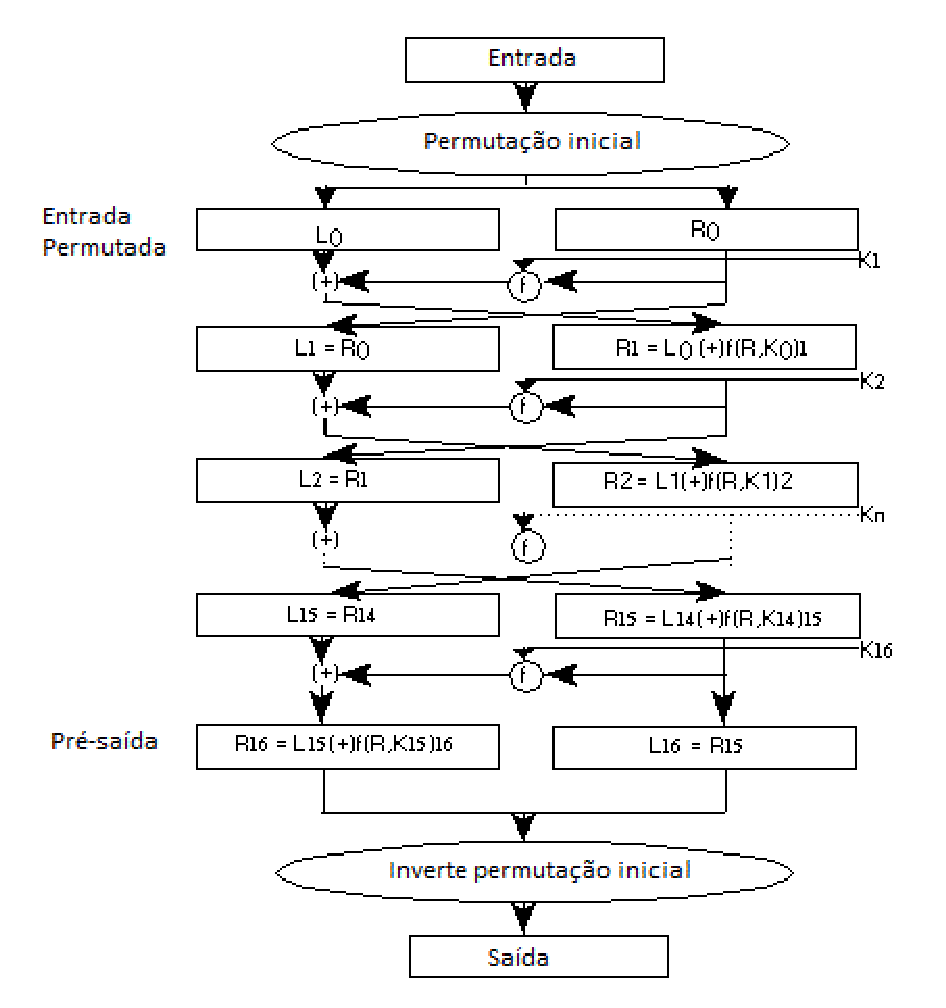
\includegraphics[scale=0.8]
		{figuras/des_cipher.eps}
		\caption[Cifra \textit{DES}]{Cifra DES\protect\footnotemark} 
		\label{cifra-des}
\end{figure}
\footnotetext{Disponível e adaptado de: \url{http://www.eventid.net/show-DocId-19.htm}}

Esse algoritmo utiliza chave de 56 \textit{bits} e opera em blocos de dados de 64 \textit{bits}. A fase de inicialização é feita uma permutação do bloco de dados iniciais. O outro passo da fase de inicialização é dividir o bloco de dados em blocos de 32 \textit{bits}. 

Depois dessa divisão, as operações são executadas no bloco que fica a direita como mostrado na Figura \ref{cifra-des}. Esse algoritmo introduz dois atributos: confusão e difusão. O atributo de confusão é feito por uma camada de substituição \textit{S-box}. A camada de permutação é feita pela \textit{P-box} e é responsável pelo atributo de difusão na cifra. O resultado dessas duas operações no bloco do lado direito é feito um ou-exclusivo com o lado esquerdo e isso resulta no lado direito do próximo \textit{round}. Essas operações se repetem em todos os 16 \textit{rounds}. No último passo é realizada a inversão da permutação inicial. No Pseudo-código \ref{des-pseudo-code} pode ser demonstrado os passos acima descritos.

    \begin{lstlisting}[caption={Pseudo-código DES}, label=des-pseudo-code]
void desCipher(char plainBlock[64], char roundKeys[56], char cipherBlock[64]){

  char tempBlock[64] = permutation(plainBlock, initialPermutation)
  char leftBlock[32] = split(0,32,tempBlock)
  char rightBlock[32] = split(32,64,tempBlock)
  for(i = 0; i < 16; i++){
	sbox = sbox(rightBlock)  
	pbox = pbox(sbox)
	rightBlock = pbox ^ leftBlock
  }
  
  tempBlock = combination(leftBlock, rightBlock)
  cipherBlock = permutation(tempBlock, finalPermutation)
}
    \end{lstlisting}


\subsubsection{Algoritmo AES}

O algoritmo \textit{AES} foi inventado com o intuito de dar mais segurança ao processo de criptografia e foi adotado como algoritmo padrão pelo \textit{NIST}. Esse algoritmo, ao contrário do \textit{DES}, não utiliza a cifra de \textit{feistel} como base. 

\begin{figure}[h]
	\centering
	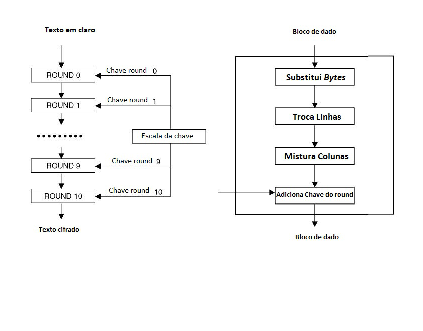
\includegraphics[scale=2]
		{figuras/aes_cipher.eps}
		\caption[Cifra\textit{AES}]{Cifra AES\protect\footnotemark} 
		\label{cifra-aes}
\end{figure}
\footnotetext{Disponível e adaptado de: \url{http://www.ecs.umass.edu/ece/koren/FaultTolerantSystems/simulator/AES-L/help.html}}

%rever
O algoritmo \textit{AES} utiliza chaves com tamanhos variáveis e essas dependem da quantidade de \textit{rounds} que são utilizados. Exemplo é que para 10 \textit{rounds} o tamanho da chave que deve ser utilizado é de 128 \textit{bits}, para 12 \textit{rounds} o tamanho da chave é de 192 \textit{bits} e para 14 \textit{rounds} o tamanho da chave correspondente é 256 \textit{bits}. Isso é feito, pois para cada \textit{round}, um pedaço da chave é utilizado.

O tamanho do bloco que é utilizado é de 128 \textit{bits} e é chamado de estado. O bloco de estado é dividido em uma matriz 4 $\times$ 4. A forma como cada \textit{round} é feita pode ser vista na Figura \ref{cifra-aes}. Todos os \textit{rounds} são idênticos, com exceção do último \textit{round}. Em cada \textit{round} a operação de substituição com a função \textit{S-box} é feita e essa operação introduz confusão a cifra. Outra operação que é realizada em cada \textit{round} é a de permutação com a função de \textit{P-box} e introduz difusão a cifra. A permutação é composta pela mistura de colunas e linhas da matriz que o bloco foi dividido. A diferença entre o último \textit{round} e os anteriores é o passo de mistura das colunas, o documento de proposta de algoritmo explica o porque: Para que a cifra e o inverso da mesma sejam mais similares em estrutura, a camada de mistura de colunas do último \textit{round} é diferente das camadas de permutações de \textit{rounds} anteriores \cite{aes-proposal}.

    \begin{lstlisting}[caption={Pseudo-código AES}, label=aes-pseudo-code]
void aesCipher(char plainState[128], char roundKeys[rounds], char cipherState[128]){

  char matrix[4][4] = transformInMatrix(plainState)
  for(i = 0; i < rounds; i++){
	char tempMatrix[4][4] = sBox(matrix)   
	tempMatrix = shiftRows(tempMatrix) 
	tempMatrix = mixColumns(tempMatrix)
	matrix = AddKeys(tempMatrix, roundKeys[i])
  }
  tempMatrix = shiftRows(matrix)
  cipherBlock = AddKeys(tempMatrix, roundKeys[round])
}
    \end{lstlisting}

\subsection{Cifra de Fluxo}
\label{stream-cipher}

%rever virgulas
Os algoritmos que utilizam a cifra de fluxo o fazem \textit{bit} a \textit{bit} ou \textit{byte} a \textit{byte}. Uma das vantagens da cifra de fluxo, em relação a cifra de bloco, é seu desempenho superior e, por esse motivo, é muito utilizado em sistemas de redes, tais como \textit{bluetooth}, \textit{SSL} e outros. 

Outra vantagem é a possibilidade de transformar uma cifra de bloco em cifra de fluxo. Para isto basta definir que o tamanho do bloco seja um \textit{bit} ou um \textit{byte}. Alguns dos algoritmos de fluxo mais populares, que hoje cobrem mais de 80\% do mundo na telecomunicação e \textit{cyber space}, são: A5/1, A5/2, E0 e RC4 \cite{majid-mohd}.

A Figura \ref{stream-cipher-functioning} representa o  funcionamento da cifra de fluxo, que funciona a partir de um gerador de \textit{keystream}\footnote{Sequência de caracteres aleatórios ou pseudo-aleatórios que são utilizados para a cifra de fluxo.}, que é gerado a partir de uma chave. Este \textit{keystream} é utilizado para cifrar os \textit{bits} do texto em claro. Para decifrar, o mesmo \textit{keystream} deve ser gerado para que possa fazer a operação ou-exclusivo com os \textit{bits} do texto cifrado.

\begin{figure}[h]
\centering
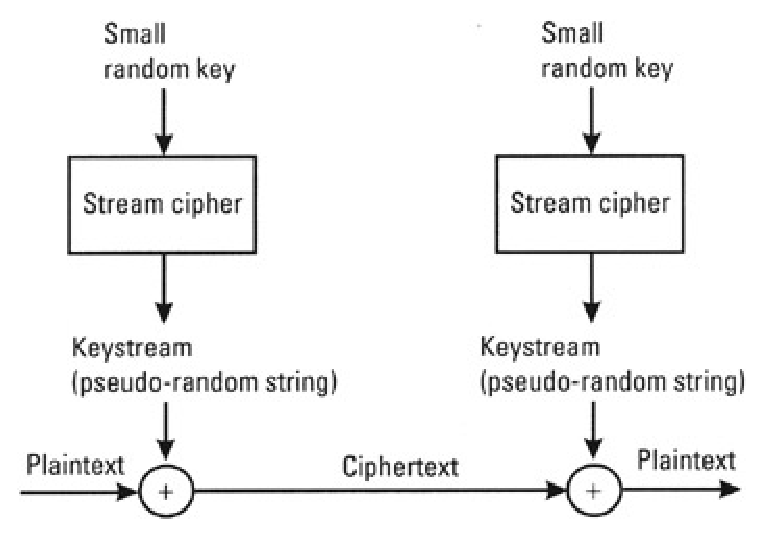
\includegraphics[keepaspectratio=true,scale=0.9]
    {figuras/stream_cipher.eps}
    \caption[Funcionamento da cifra de fluxo]{Funcionamento da cifra de fluxo\protect\footnotemark} 
    \label{stream-cipher-functioning}
\end{figure}
\footnotetext{Disponível e adaptado de: \url{http://www.globalspec.com/reference/81191/203279/2-6-stream-ciphers}}

\subsubsection{Algoritmo A5/1}
\label{algorithm-a51}

Principal algoritmo usado no mundo para a comunicação \textit{GSM}, foi desenvolvido em 1987 e teve seu funcionamento mantido em segredo e somente em 1999 foi revelado por engenharia reversa. Consiste de três \textit{Linear Feedback Shift register} ou \textit{LFSR} binários R1, R2 e R3. Um \textit{LFSR} é um registrador que mantém valores de estado anterior e é atualizado por uma função que normalmente é um ou-exclusivo. Esses registradores são atualizados com cronômetro irregular, o que significa que a forma de atualização dos três registradores acontecem de forma independente. 

\begin{figure}[h]
\centering
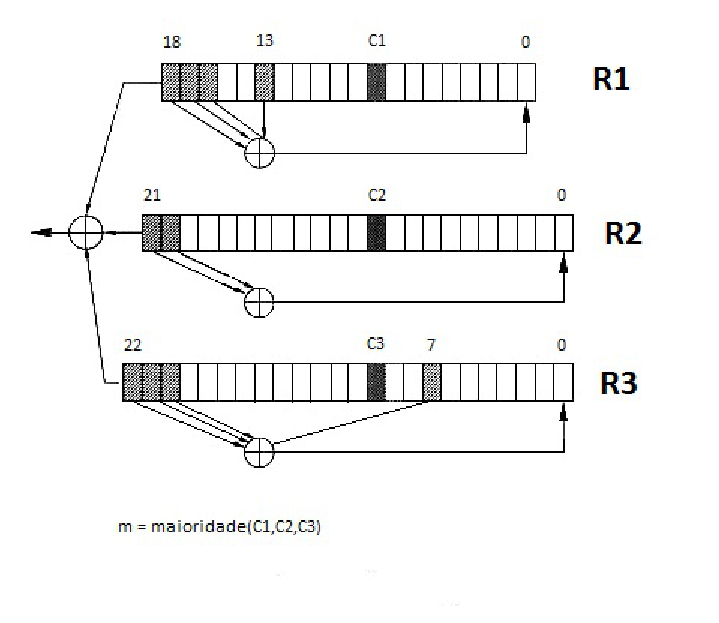
\includegraphics[keepaspectratio=true,scale=0.9]
    {figuras/a5_1.eps}
    \caption[Estrutura do algoritmo A5/1]{Estrutura do algoritmo A5/1\protect\footnotemark} 
\end{figure}
\footnotetext{Disponível e adaptado de: \url{http://cryptome.info/0001/a51-bsw/a51-bsw.htm}}

Cada registrador contém \textit{bits} importantes para a criptografia e suas posições são predeterminadas. São os \textit{bits} do \textit{clocking} e \textit{tapping}, que estão definidos na tabela \ref{important-bits}. Os registradores tem tamanhos diferentes sendo que, o R1 tem 19 \textit{bits}, o R2 tem 22 \textit{bits} e o R3 tem 23 \textit{bits}. O algoritmo tem como entradas a chave secreta \textit{Kc}, que tem 64 \textit{bits}, e um vetor de inicialização de 22 bits composto do \textit{frame number}. O \textit{keystream}, de 228 \textit{bits}, é a saída do processo, sendo que os primeiros 114 \textit{bits} são o \textit{keystream} de \textit{downlink} e os outros 114 \textit{bits} são o \textit{keystream} de \textit{uplink}. Cada ciclo no algoritmo é composto por passos específicos em cada registrador:

\begin{table}[h]
\centering
	\begin{tabular}{c c c}
	\toprule
		Registrador & \textit{Clocking Bits} & \textit{Tapping Bits} \\ \hline
		R1 & 8 & 13, 16, 17, 18 \\ \hline
		R2 & 10 & 20,21 \\ \hline
		R3 & 10 & 7,20,21,22 \\ \hline	
	\end{tabular}
	\caption{\textit{Bits} importantes do algoritmo A5/1}
	\label{important-bits}
\end{table}

A operação de ou-exclusivo é realizada entre os \textit{tapping bits} de cada registrador. Utilizando a regra de maioridade\footnote{Essa regra funciona da seguinte maneira, os três \textit{clocking bits} de cada registrador são comparados e os registradores que tiverem os \textit{bits} que teve maior ocorrência na comparação são acionados, por exemplo o R1 tem \textit{bit} 1, o R2 tem \textit{bit} 0 e o R3 tem \textit{bit} 1, então o \textit{bit} com maior ocorrência é o 1, sendo assim somente os registradores R1 e R3 são acionados naquele ciclo.} com os \textit{clocking bits}. O registrador é acionado se o valor contido no \textit{clocking bits} for igual ao resultado da regra de maioridade e então os \textit{bits} do registrador são deslocados da direita para a posição mais a esquerda do registrador.

\begin{lstlisting}[caption={Pseudo-código A5/1}, label=a51-pseudo-code]
void a51Generation(key key[64]){

  int i;
  for(i = 0; i < 64; i++){
  	R1[0] = R1[0] ^ key[i]
	R2[0] = R2[0] ^ key[i]
	R3[0] = R3[0] ^ key[i]  
  }

  registers R1[19] ,R2[22], R[23]
  
  resultR1 = R1[13] ^ R1[16] ^ R1[17] ^ R1[18]
  resultR2 = R2[20] ^ R2[21]
  resultR3 = R3[7] ^ R3[20] ^ R3[21] ^ R3[22]
  
  clockingBit = marjorityRule(R1[8], R2[10], R3[10])
  if(R1[8] == clockingBit){
  	deslocateToTheLeft(resultR1)
  }else if(R2[10] == clockingBit){
    deslocateToTheLeft(resultR2)
  }else if(R3[10] == clockingBit){
    deslocateToTheLeft(resultR3)
  }
  
  output = R1[18] ^ R2[21] ^ R3[22]
}
    \end{lstlisting}

Se o registrador for acionado, então o resultado do ou-exclusivo do primeiro passo deve ser passado para a posição zero do registrador correspondente.

Finalmente, a saída é definida pelo ou-exclusivo dos \textit{bits} dos registradores nas posições: R1[18], R2[21] e R[22]. Para a fase de iniciação é utilizada a chave de 64 \textit{bits} e passa de \textit{bit} por \textit{bit} fazendo ou-exclusivo da posição 0 de cada registrador com o \textit{bit} da chave. O algoritmo ignora o resultado das primeiras 100 execuções e depois retorna os \textit{bits} do \textit{keystream} a cada 228 ciclos, gerando os 228 \textit{bits} de saída.

\subsubsection{Algoritmo A5/2}
\label{algorithm-a52}

Esse algoritmo foi desenvolvido por motivos de restrições de exportação do A5/1 e tem uma estrutura similar ao A5/1, com algumas exceções, como por exemplo: o A5/2 utiliza 4 registradores. Outra diferença é o fato que o \textit{clocking} dos registradores R1, R2 e R3 são acionados baseados na regra de maioridade do R4. Ou seja, cada registrador é acionado dependendo dos \textit{bits} do registrador R4. 

\begin{table}[h]
\centering
	\begin{tabular}{c c c c}
	\toprule
	Registrador & \textit{Clocking Bits} & \textit{Tapping Bits} & \textit{Bits} utilizados na função maioridade \\ \hline
		R1 & 8 & 13, 16, 17, 18  & 12, 14*\protect\footnotemark , 15\\ \hline
		R2 & 10 & 20, 21 & 9, 13, 16*\\ \hline
		R3 & 10 & 7, 20, 21, 22 & 13*, 16, 18\\ \hline	
		R4 & 3, 7, 10 & - & -\\ \hline
	\end{tabular}
	\caption{\textit{Bits} importantes do algoritmo A5/2}
\end{table}
\footnotetext{\textit{Bit} complementar}
\begin{figure}[h]
\centering
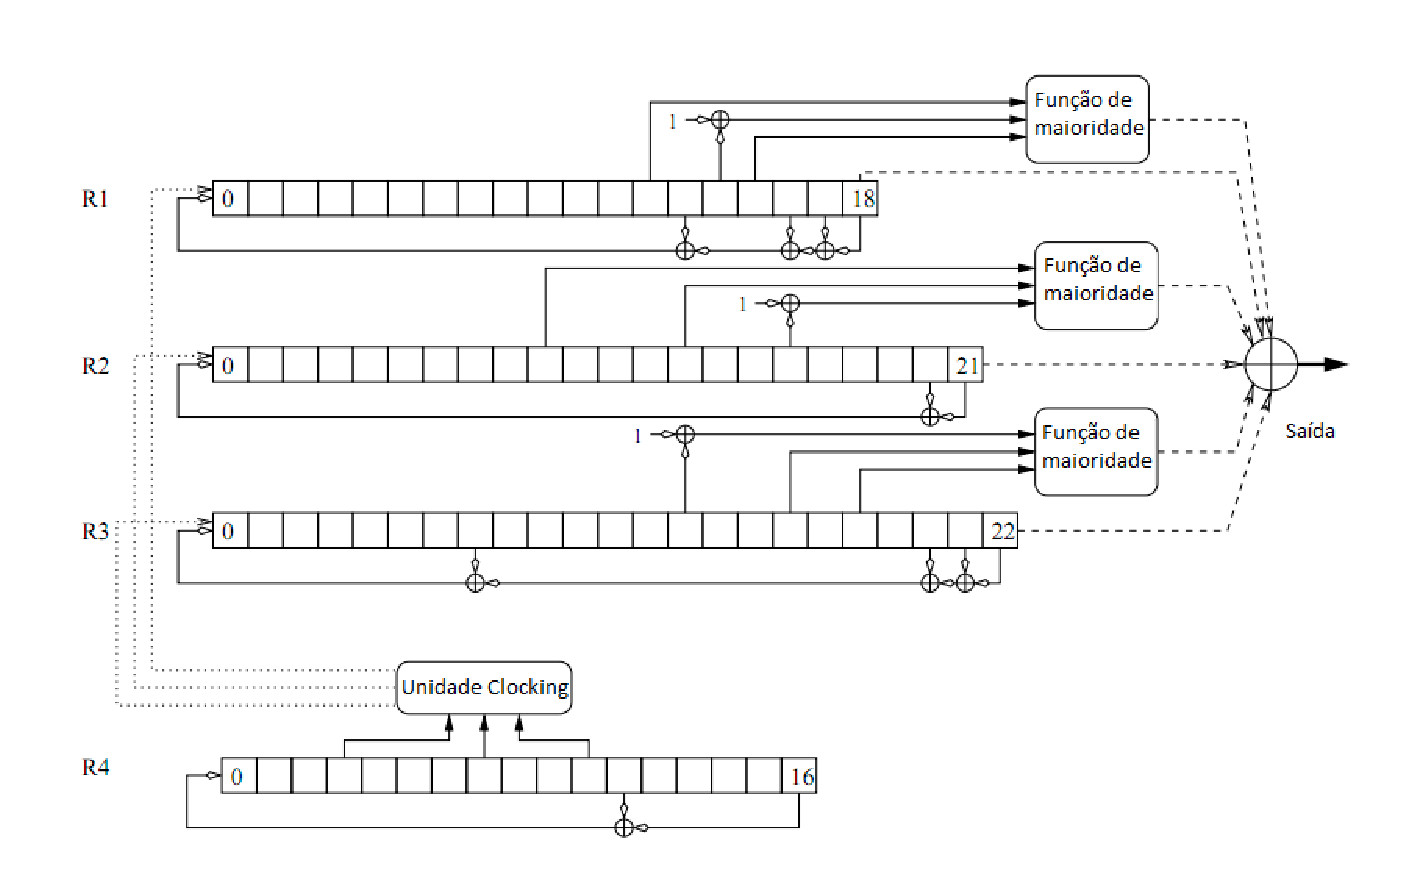
\includegraphics[keepaspectratio=true,scale=0.5]
    {figuras/a5_2.eps}
    \caption[Estrutura do algoritmo A5/2]{Estrutura do algoritmo A5/2\protect\footnotemark } 
\end{figure}
\footnotetext{Disponível e adaptado de: \url{http://blog.cryptographyengineering.com/2012/02/sattelite-phone-encryption-is-terrible.html}}

Caso o resultado da regra da maioridade dos \textit{clocking} \textit{bits} do R4 seja igual ao do \textit{bit} que se encontra na posição 3 então o registrador R2 é acionado, caso seja igual ao \textit{bit} que se encontra na posição 7 então o registrador R3 é acionado e se for igual ao \textit{bit} que está na posição 10 então o registrador R1 é acionado. Depois que os registradores são acionados, então o registrador R4 é acionado também. A saída desse algoritmo é feita da forma demonstrada pelo Pseudo-código \ref{a52-pseudo-code}

\begin{lstlisting}[caption={Pseudo-código A5/2}, label=a52-pseudo-code]
void a52Cipher(key key[64]){

  registers R1[18] ,R2[21], R3[22], R4[16]

  clockingBit = marjorityRule(R4[3], R4[7], R4[10])
  
  resultR1 = 0  
  resultR2 = 0  
  resultR3 = 0
  if(clockingBit == R4[3]){
  	// R2 
  	complement = 1 ^ R2[16]
  	resultR2 = marjorityRule(complement, R2[9], R2[13]) ^ R2[21]
  	deslocateToLeft(R2, R2[21] ^ R2[20])
  
  } else if(clockingBit == R4[7]) {
  // R3
  	complement = 1 ^ R3[13]
  	resultR3 = marjorityRule(complement, R3[16], R3[18]) ^ R3[22]
  	deslocateToLeft(R3, R3[22] ^ R3[21] ^R3[20])  
  
  } else {
  //R1
    complement = 1 ^ R1[14]
  	resultR1 = marjorityRule(complement, R1[12], R1[15]) ^ R1[18]
  	deslocateToLeft(R1.R1[18] ^ R1[17] ^R1[16] ^ R1[13]) 
  }
  
  deslocateToLeft(R4, R4[16] ^ R4[11])
  
  output = resultR1 ^ resultR2 ^ resultR3
}
    \end{lstlisting}

%rever, escrever em forma de parágrafo??
\begin{enumerate}
	\item É calculado o complementar do \textit{bit} da posição especificada de cada registrador.
	\item Em cada registrador é utilizado a regra da maioridade para dois \textit{bits} e o complementar do \textit{bit} calculado anteriormente. 
	\item É feito um ou-exclusivo do resultado do item anterior com o \textit{bit} mais significativo do registrador de cada registrador.
\end{enumerate}


\subsubsection{Algoritmo E0}
\label{algorithm-e0}

Utilizado para proteger informações que utilizam a tecnologia \textit{bluetooth}. O principal objetivo dessa tecnologia é conectar dois aparelhos para transferência de algum tipo de informação.

\begin{figure}[h]
	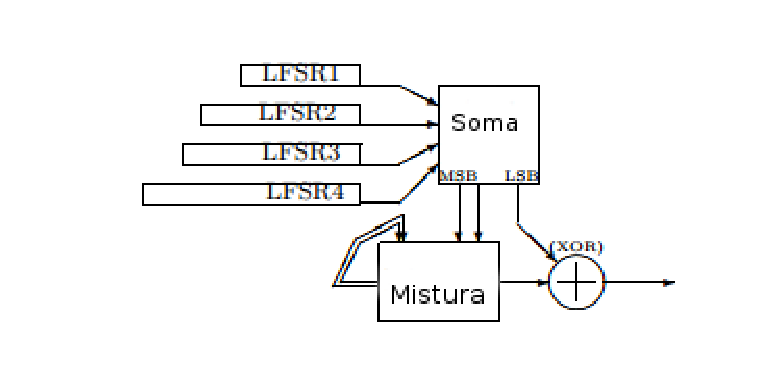
\includegraphics[scale=1]{figuras/e0.eps}
	\caption{Estrutura do algoritmo E0\cite{fluhrer-lucksl}}
	\label{e0-structure}
\end{figure}

O algoritmo também é baseado no uso de registradores e a saída é gerada em ou-exclusivo de \textit{bits} de cada registrador. Nesta estrutura, são utilizados 4 registradores com tamanhos 25, 31, 33 e 39 \textit{bits}. O sistema da geração do \textit{keystream} é um pouco diferente, a cada \textit{clock tick} todos os registradores são acionados e é feito um ou-exclusivo da saída de cada um. A operação é descrita a seguir:

\begin{lstlisting}[caption={Pseudo-código E0}, label=e0-pseudo-code]
void e0Cipher(key key[64]){

  registers R1[25] ,R2[31], R3[33], R4[39]


  while(clockTick) {
  	result = sum(R1,R2, R3, R4)
  	char finiteStateMachine[3] = msb(result)
  	output = finiteStateMachine ^ lsb(result)
  }
}
    \end{lstlisting}

\subsubsection{Algoritmo RC4}
\label{algorithm-rc4}

Projetado em 1987 por Ron Rivest, é muito utilizado em sistemas de redes como TLS/SSL e WEP por conta de sua simplicidade e alto desempenho. Tem tamanho de chave variável e se baseia em permutações aleatórias. Utiliza um gerador de números aleatórios e as permutações são realizadas sobre esses números aleatórios.

O funcionamento do algoritmo é realizado com uma leitura do texto em claro feita a cada \textit{byte} e cada \textit{byte} produz um \textit{byte} de texto cifrado. Seu funcionamento está ligado a um gerador de \textit{keystream}, ou seja, utilizando como entrada uma chave é criada uma sequência de números aleatórios.

O RC4 é dividido em três passos fundamentais: a inicialização, geração aleatória de \textit{bytes} e cifração.

\begin{description}

	\item [Inicialização] RC4 aceita chaves de tamanho variáveis. Na fase de inicialização, o vetor S é inicializado com valores iniciais seguindo o código mostrado a seguir:
	
    \begin{lstlisting}[caption={Código 
Inicialização}, label=inicialization]
typedef struct RC4{
	int i;
	int j;
	char state[255];
}

void rc4Initializer(RC4 * params, char key[], unsigned char * temp[255] ){

  int i,j = 0;
  size_t keylen = strlen(key);
  for(i = 0; i <= 255; i++){
    params->state[i] = i;
    temp[i] = key[i % keylen];
  }
  return temp;
}
    \end{lstlisting}

Como pode ser visto no código anterior, um vetor temporário de 256 \textit{bytes} é criado juntamente com a inicialização do vetor de 256 \textit{bytes} \textit{state}. O vetor \textit{temp} é inicializado com os valores da chave K. Se a chave tem tamanho 256 \textit{bytes}, então \textit{temp} é igual a K. Se K for menor que 256 \textit{bytes} então a chave é repetida até preencher as 256 posições de \textit{temp}.

Após a inicialização do vetor \textit{temp}, é feita uma permutação inicial utilizando variáveis de controle \textit{i} e \textit{j} e é realizada obedecendo o código abaixo:

    \begin{lstlisting}[caption={Código Permutação Inicial}, label=initialPermutation]
void intialPermutation(RC4 * params, char key[], unsigned char * temp[255]){

  int j = 0;
  unsigned char swap;
  for(i = 0; i <= 255; i++) {
    j = (j + params->state[i] + temp[i]) % 256;
    swap = params->state[j];
    params->state[j] = params->state[i];
    params->state[i] = swap;
  }

  params->i = 0;
  params->j = 0;
}
    \end{lstlisting}

	\item [Geração Aleatória de \textit{bytes}] Após a permutação inicial, a geração de \textit{bytes} é feita utilizando de permutações aleatórias do vetor \textit{state}. Essa geração utiliza das variáveis de controle \textit{i}, \textit{j} e \textit{k}. Essa geração é realizada a cada cifração realizada pelo algoritmo. A geração é feita da seguinte forma:
	
    \begin{lstlisting}[caption={Código Geração Aleatório de \textit{bytes}}, label=randomGeneration]
char rc4Generator(RC4 * params){

  unsigned char t;
  unsigned char k;
  unsigned char swap;
  params->i = (params->i + 1) % 256;
  params->j = (params->j + params->state[params->i]) % 256;
  swap = params->state[params->j];
  params->state[params->j] = params->state[params->i];
  params->state[params->i] = swap;
  t = (params->state[params->i] + params->state[params->j]) % 256;
  k = params->state[t];

  return k;
}
    \end{lstlisting}

	\item [Cifração] Para a fase de cifração é preciso que se obtenha um \textit{byte} da função de gerador aleatório. A cifração desse algoritmo é feita com a operação ou-exclusivo entre o \textit{byte} proveniente do gerador e o \textit{byte} correspondente do texto em claro.

    \begin{lstlisting}[caption={Código Cifração de \textit{bytes}}, label=encryption]
char rc4Encryption(RC4 * params, char plainText){

	byteToCipher = rc4Generator(params);
	return plainText ^ byteToCipher;
}
    \end{lstlisting}

\end{description}


%
\section{Criptografia Assimétrica}
\label{assymmetric-cryptography}

%
A criptografia assimétrica é usada principalmente para cifrar dados pequenos. Um dos principais usos é a assinatura digital e para realizar a troca de chaves de forma segura. Esse tipo de criptografia está associada à criptografia de chave pública. Nela é estabelecido que um par de chaves (chave pública e privada) sejam usadas para a cifração e decifração da mensagem. 

%
O funcionamento é simples. Bob tem suas duas chaves e disponibiliza sua chave pública de forma que qualquer pessoa que tenha interesse em lhe enviar uma mensagem criptografada, utilize sua chave pública. Quando Bob recebe a mensagem cifrada, é realizada a decifração dessa mensagem utilizando sua chave privada.

%
Alguns dos algoritmos mais conhecidos são o \textit{Elgamal} e o \textit{Diffie-Hellman}. O algoritmo \textit{RSA} foi o primeiro algoritmo a cifrar e decifrar com sucesso utilizando o princípio da chave pública. O \textit{Elgamal} tem sua força proveniente da dificuldade de se calcular um logaritmo discreto. Com o \textit{Elgamal} pode-se realizar a assinatura digital de um documento. \textit{Diffie-Hellman} foram os visionários da chave pública, primeiramente definiram a ideia e algum tempo depois definiram um algoritmo que serve apenas para trocar uma chave secreta entre duas pessoas. 

\subsection{Algoritmo RSA}
\label{algorithm-rsa}

Tem seu nome baseado nas iniciais dos cientistas do \textit{MIT} que o inventaram: \textit{Ron Rivest, Adi Shamir} e \textit{Len Adleman}. A geração das chaves desse algoritmo é feita utilizando números primos e sua força está associada ao fato de que é fácil realizar a multiplicação de dois números primos grandes, mas é difícil a decomposição desse resultado. Portanto a chave é gerada da seguinte forma:

\begin{enumerate}
\item Dois números \textbf{p} e \textbf{q} são escolhidos de forma aleatória e são primos.
\item \textbf{p} $\neq$ \textbf{q}
\item \textbf{n} é composto pela multiplicação de \textbf{p} e \textbf{q}.
\item \textbf{e\footnote{Chave pública, para cifrar um texto.}}, tal que mdc\footnote{Operação matemática que visa descobrir o maior divisor comum entre dois ou mais números}($\phi$(n, e)) = 1
\item \textbf{d\footnote{Chave privada, para decifrar um texto }}, (e $^ {(-1)}$) $\times$ ($\bmod$ $\phi$(n)) 
\end{enumerate}

%
A chave pública \textbf{e}  é usada para cifrar a mensagem e a chave privada \textbf{d} é usada para decifrar. O método de cifra é simples, o texto é tratado como um conjunto de inteiros e a cada inteiro é feito o seguinte cálculo:

\begin{description}
\item [Cifrar]
C = M $^ e$ $\bmod$ n. Sendo que M é o inteiro correspondente a parte do texto em claro e n o resultado da multiplicação dos dois números primos selecionados na confecção  das chaves, C é o texto cifrado e \textbf{e} é a chave pública. 
\item [Decifrar]
M = C $^ d$ $\bmod$ n. Sendo que C é o texto cifrado, M o texto em claro e \textbf{d} é a chave privada.
\end{description}

\begin{lstlisting}[caption={Pseudo-código RSA}, label=rsa-pseudo-code]
int phi(p, q){
	return (p - 1) * (q - 1)
}

void rsaCipher(key key[64], char plainText){
	int p = getBigPrime()
	int q = getBigPrime()
	
	while( p == q){
		q = getBigPrime()
	}
	
	int n = p * q
	
	e = mdc(phi(n, e)
	while(e != 1){
		e = mdc(phi(n, e))
	}
	
	d = pow(e, (-1)) % (n - 1)
	
	c = pow(plainText, e) % n
	
}
    \end{lstlisting}

%
\section{Criptoanálise}
\label{cryptanalysis}

Estudo que tem como objetivo a criação de técnicas e métodos que ajudam a obter o texto em claro a partir de um texto cifrado sem ter a devida autorização. Conforme a criptografia cresceu e seus estudos se aprofundaram, os estudos da criptoanálise também cresceram. Abaixo algumas técnicas de criptoanálise.

\subsection{Força Bruta}
\label{brute-force}

Esse ataque visa procurar por exaustão a chave usada para cifrar a mensagem. Para isso testa-se todas as possibilidades de chave e analisa o texto produzido. 

É eficiente para chaves pequenas, pois a quantidade de chaves possíveis é pequena. Por se tratar de uma procura pela chave, esse método pode ser aplicado em diferentes tipos de algoritmo criptográfico.

\begin{table}[h]
\centering
	\begin{tabular}{ c c }
	\toprule
		Tamanho da chave & Tempo para quebrar \\ \hline
		32 & 2.15 milissegundos \\ \hline
		56 & 10.01 horas \\ \hline
		128 & 5.4 X $ 10 ^{18}$ anos \\ \hline
		168 & 5.9 X $ 10 ^{30}$ anos \\ \hline
	\end{tabular}
\caption[{Tempo gasto para encontrar chaves}] {Tempo gasto para encontrar chaves adaptado de \cite{william-stallings}}
\end{table}

\subsection{Análise de Frequência}
\label{frequency-analysis}

Esse método visa analisar a frequência de ocorrência de cada caractere de um texto cifrado. Existem diversos estudos que indicam a frequência média de ocorrência de cada letra em um texto. 

\begin{table}[h]
\centering
\begin{tabular}{ c c | c c }
\toprule
	Letra & Frequência no texto & Letra & Frequência no texto \\ \hline
	a & 8.167 & n & 6.749 \\ \hline
	b & 1.492 & o & 7.507 \\ \hline
	c & 2.782 & p & 1.929 \\ \hline
	d & 4.253 & q & 0.095 \\ \hline
	e & 12.702 & r & 5.987 \\ \hline
	f & 2.228 & s & 6.327 \\ \hline
	g & 2.015 & t & 9.056 \\ \hline
	h & 6.094 & u & 2.758 \\ \hline
	i & 6.966 & v & 0.978 \\ \hline
	j & 0.153 & w & 2.360 \\ \hline
	k & 0.772 & x & 0.150 \\ \hline
	l & 4.025 & y & 1.974 \\ \hline
	m & 2.406 & z & 0.074 \\ \hline
\end{tabular}
\caption[{Frequência média de letras em um texto em inglês}]{Frequência média de letras em um texto em inglês \cite{robert-lewand}} 
\end{table}

A ideia é identificar as frequências do texto cifrado e substituir as letras a medida que for identificado, até conseguir produzir um texto coeso.

Esse é o método que o algoritmo proposto neste trabalho visa dificultar, visto que sua aplicação pode ser utilizada em diversos tipos de algoritmos criptográficos e seus resultados podem ser satisfatórios. Com o balanceamento das ocorrências do texto cifrado, as frequências médias conhecidas não servirão de apoio para possíveis ataques, visto que cada caractere terá a mesma frequência de ocorrência.